\section{Übung 108}
\begin{minipage}[t]{0.33\textwidth}
	$\underline{\text{Gegeben:}}$
	\begin{itemize}
		\item $h = \SI{30}{\centi \meter}= \SI{0,3}{\meter}$
		\item  $m_{\text{OK}} = \SI{485}{\kg}$
		\item $\rho_{GG} = \SI{7,2}{\kg \per \liter}=\SI{7200}{\kg \per \kmeter}$
		\item $D = \SI{825}{\milli \meter} = \SI{0,825}{\meter}$
		\item $d = \SI{270}{\milli \meter} = \SI{0,270}{\meter}$
		\item $s = \SI{100}{\milli \meter} = \SI{0,1}{\meter}$
	\end{itemize}
\end{minipage}
\begin{minipage}[t]{0.33\textwidth}
	$\underline{\text{Gesucht:}}$
	\begin{itemize}
		\item $\overrightarrow{F}_{\text{Schraube}}$
	\end{itemize}
\end{minipage}
\begin{minipage}[t]{0.33\textwidth}
	$\underline{\text{Verwendete Formeln:}}$
		\begin{align}
			\overrightarrow{F} &= m*g \\
			&= \rho*g*A*h
		\end{align}
		\begin{equation}
			A = \frac{\pi}{4}*\left(D^2-d^2\right)
			\end{equation}
\end{minipage}

\vspace*{5mm}

\textit{Zur Erinnerung: }
\begin{flalign*}
	\overrightarrow{F}_{\text{Auftrieb}} &= V*g*\rho
\end{flalign*}

\begin{figure}[h!]
	\centering
	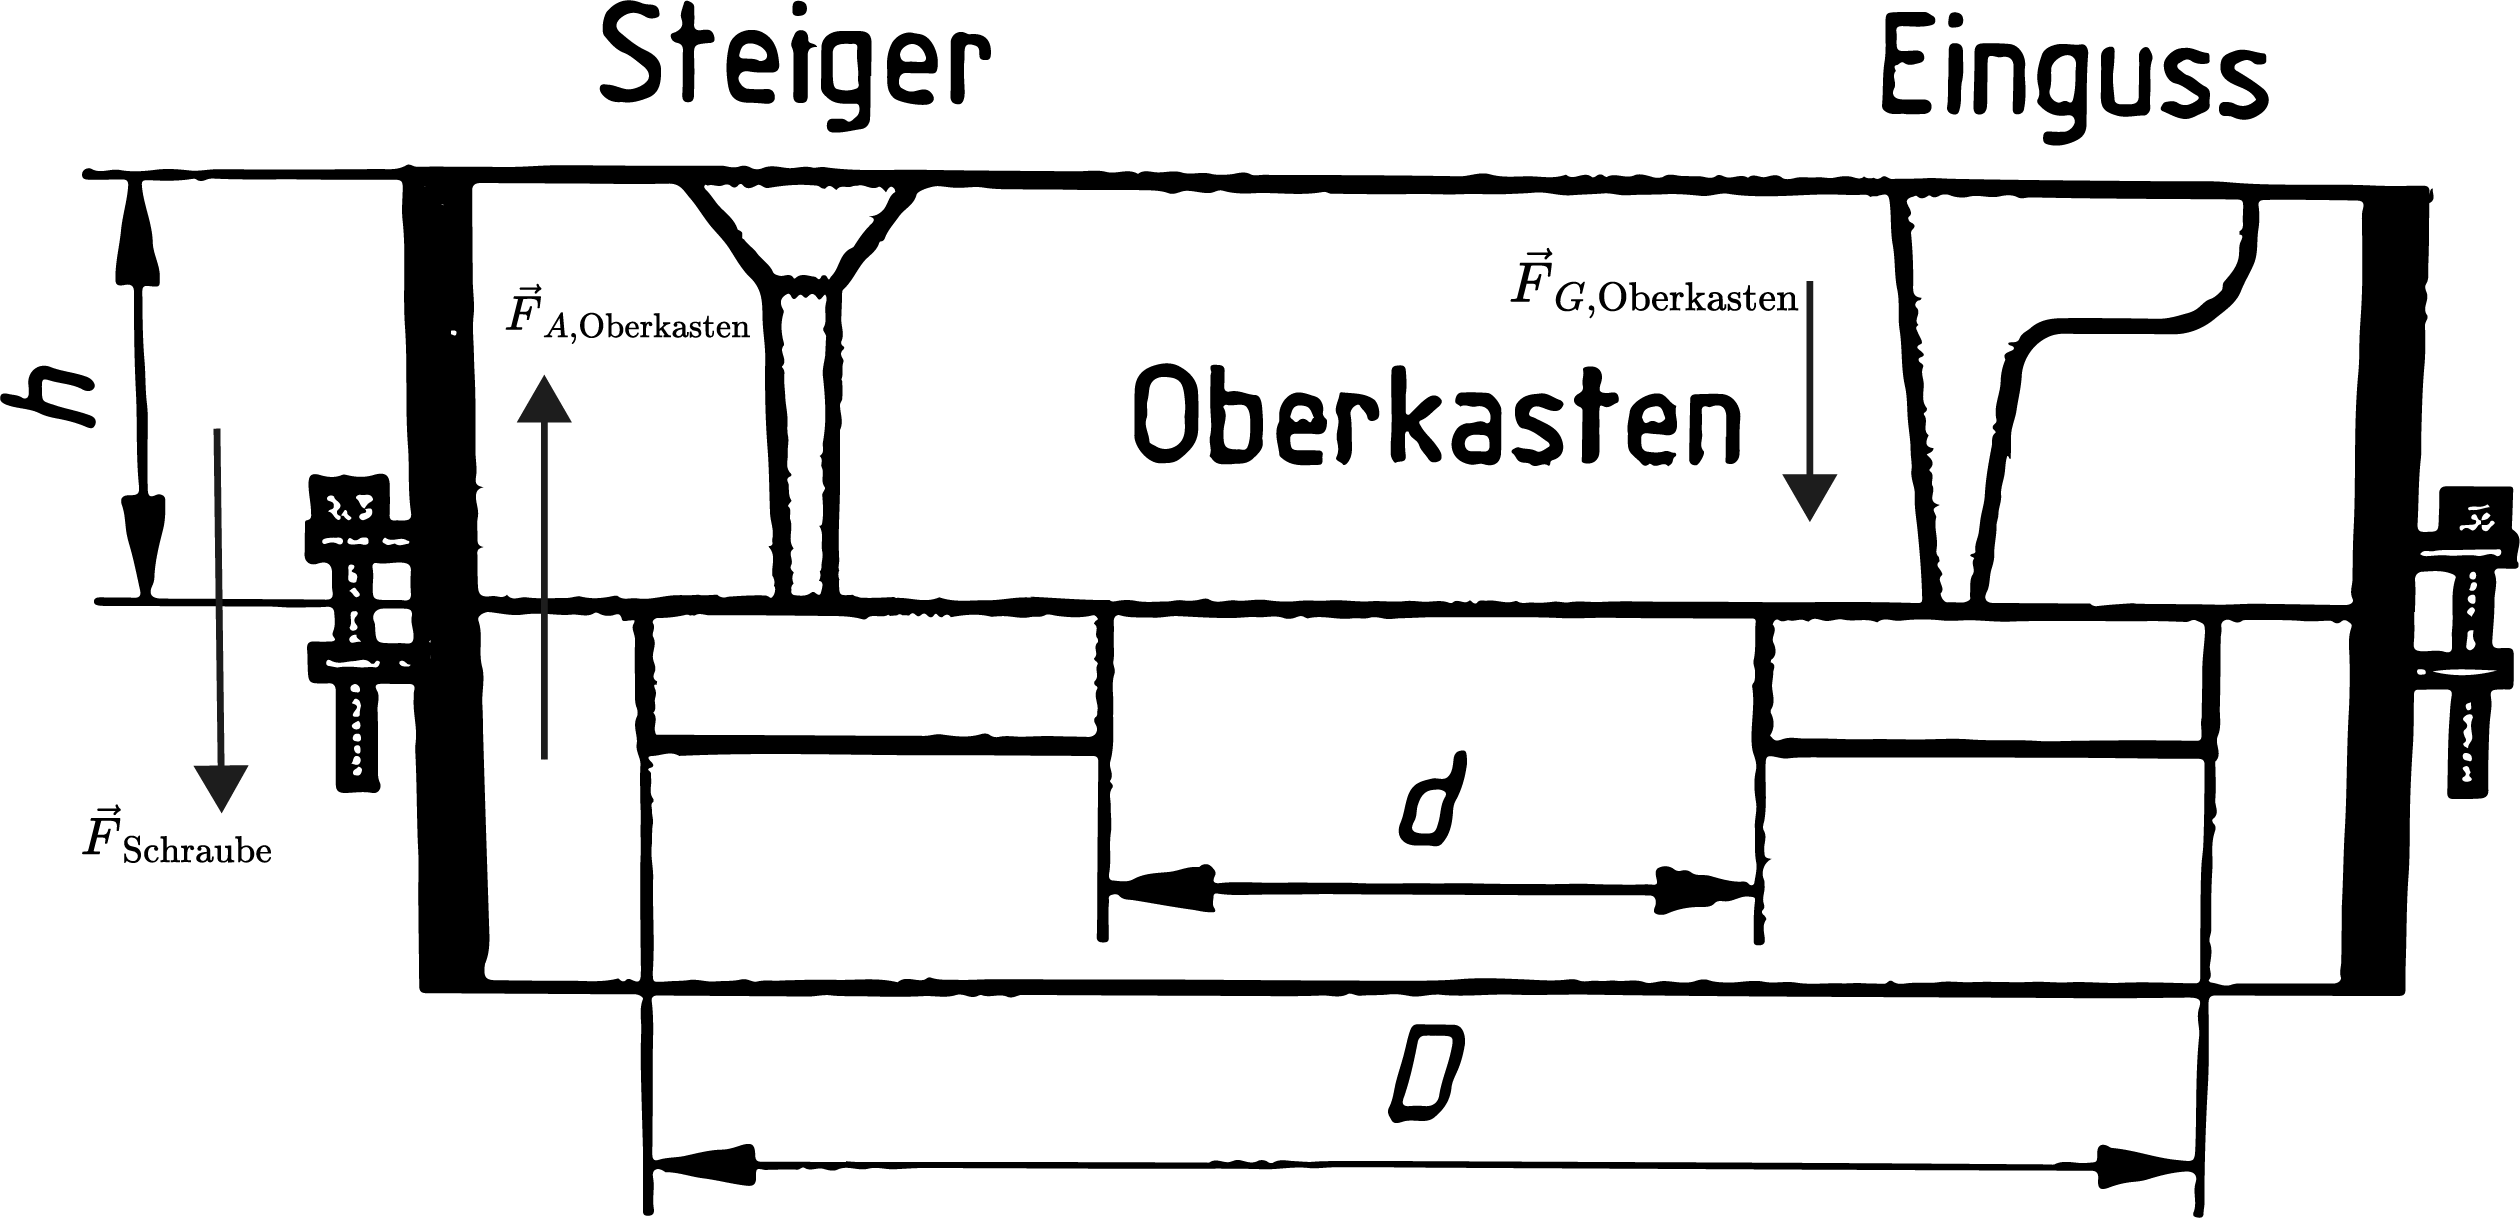
\includegraphics[width=0.8\textwidth]{u108}
\end{figure}
\FloatBarrier
%Ende

\begin{flalign}
	\overrightarrow{F}_{G, \text{Oberkasten}} &= m*g\\
	&= \SI{485}{\kg}*\SI{9,81}{\g}\\
	&= \underline{\SI{4747,85}{\newton}}
\end{flalign}
\begin{flalign}
	A_{\text{proj}}&= \frac{\pi}{4}*\left(D^2-d^2\right)\\
	&= \frac{\pi}{4}*\left(\SI{0,825}{\meter}^2-\SI{0,270}{\meter^2}\right)\\
	&= \underline{\SI{0,477}{\smeter}}
\end{flalign}
\begin{flalign}
	\overrightarrow{F}_{A, \text{Oberkasten}} &= A_{\text{proj}}*\rho_{GG}*g*h\\
	&= \SI{0,477}{\smeter}*\SI{7200}{\kg\per \kmeter}*\SI{9,81}{\g}*\SI{0,3}{\meter}\\
	&= \underline{\SI{10107,4}{\newton}}
\end{flalign}
\begin{flalign}
	\overrightarrow{F}_{A, \text{Oberkasten}} &= A_{\text{proj}}*\rho_{GG}*g*h\\
	&= \SI{0,477}{\smeter}*\SI{7200}{\kg\per \kmeter}*\SI{9,81}{\g}*\SI{0,3}{\meter}\\
	&= \underline{\SI{10107,4}{\newton}}
\end{flalign}
\begin{flalign}
	\overrightarrow{F}_{\text{Schraube}} &= 
	\overrightarrow{F}_{A, \text{Oberkasten}} -\overrightarrow{F}_{G, \text{Oberkasten}} \\
	&= \underline{\underline{\SI{5359,6}{\newton}=\SI{5,36}{\kilo \newton}}}
\end{flalign}
